\section{Multimesh concept}

\begin{example}
	Navier-Stokes-Equation:
	\begin{align*}
		\partial_t u + u \cdot \nabla u &= \nabla p + \nu \laplace u \\
		\nabla \cdot u = 0 
	\end{align*}
	with $u = (u_1,u_2,u_3)^T$ as velocity, $p$ as pressure and $\nu$ as viscosity and proper intial and boundary conditions
\end{example}

\begin{example}
	Hahn-Hilliard-Equation(phase field moduls)\\
	(e.g. seperation of two liquids)
	\begin{align*}
	\partial_t u &= \laplace u \\
	\mu &= -\varepsilon \laplace u + \frac{1}{\varepsilon}w'(u) 
	\end{align*}
	with $u$ as concentration(phase variable), $\mu$ as chemical potential and $w(u) = \frac{1}{4} (1-u^2)^2$ as the double-well potential and a small parameter $\varepsilon$.
	\begin{figure}[H]
	\center
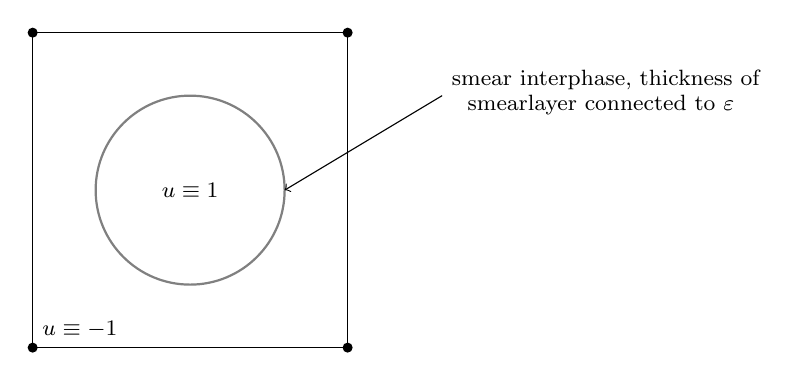
\begin{tikzpicture}[scale=4]
		
		\def \xone{0};
		\def \yone{0};		
		% first rectangle
		\coordinate (A) at (\xone,\yone);
		
        \draw (A) -- ++(0,1) -- ++(1,0)-- ++(0,-1) --cycle;
        \draw[thick,gray] (A) ++(0.5,0.5) circle (0.3cm);
        \filldraw (A)         circle (0.4pt);
        \filldraw (A) ++(1,0) circle (0.4pt);
        \filldraw (A) ++(0,1) circle (0.4pt);
        \filldraw (A) ++(1,1) circle (0.4pt);
        \fill[black,font=\footnotesize] (A)         node[above right] {$u \equiv -1$}
                                        (A) ++(0.5,0.5) node {$u \equiv 1$}
                                        (A) ++(1.3,0.85) node[right] {smear interphase, thickness of }
                                         (A) ++(1.35,0.77) node[right] {smearlayer connected to $\varepsilon$};
        \draw[-to] (A) ++(1.3,0.8) -- ++(-0.5,-0.3);
        
\end{tikzpicture}

\caption{Visualisation of motivation for pde}
\label{ch_mult_hahn_hilliard}
\end{figure}
\end{example}
\textbf{eventuell fehler in der obigen Gleichung}
\begin{example}
	for illustration , biharmonic equation
	\begin{align*}
	\laplace^2 u &= 0 \tin \Omega \\
	u &= 0 \ton \partial\Omega\\
	\frac{\partial u}{\partial n} &=0 \ton \partial \Omega
	\end{align*}
	classical solution: $u \in C^4(\Omega)\cap C^1(\bar{\Omega})$\nl
	do operator splitting and rewrite as a system:
	\begin{align*}
		\begin{rcases}
			-\laplace u + v &=0\\
			\laplace v &= 0
		\end{rcases} \tin \Omega
	\end{align*}
	variational/weak formulation: Find $(u,v) \in H^1_0(\Omega)\times H^1(\Omega)$
	\begin{align*}
		\int \limits_{\Omega} \nabla u \cdot \nabla \varphi + \int \limits_{\Omega} v\varphi &=0 \qquad \forall \varphi \in H^1\\
		\int \limits_{\Omega} \nabla v \cdot \nabla \psi &=0 \qquad \forall \psi \in H^1_0
	\end{align*}
	assume $\T^0_h, \T^1_h$ are different partitions of $\Omega$
	\begin{align*}
		V^0_h &= \left\{ v_h \in H^1: v_h|_T \in P_{\alpha},\ \forall T \in \T^0_h  \right\}\\
		V^1_h &= \left\{ v_h \in H^1_0: v_h|_T \in P_{\alpha},\ \forall T \in \T^1_h  \right\}
	\end{align*}
	$\implies$ discrete setting
	\begin{align*}
		\int \limits_{\Omega} \nabla u_h \cdot \nabla \varphi + \int \limits_{\Omega} v_h\varphi &=0 \qquad \forall \varphi \in V^0_h\\
		\int \limits_{\Omega} \nabla v_h \cdot \nabla \psi &=0 \qquad \forall \psi \in V^1_h
	\end{align*}
	Ansatz: 
	\begin{align*}
		u_h = \sum  \limits_{i=1}^{n} u_i\varphi_i,\quad v_h= \sum \limits_{i=1}^{m} v_i\psi_i
	\end{align*}
	with $\{\varphi_i,1\leq i \leq n \}$,$\{ \psi_i,\ 1 \leq i \leq m \}$ as basis of $V^0_h$ and $V^1_h$.
	\begin{align*}
		\sum \limits_{j=1}^n u_j \left( \sum \limits_{T \in \T^0_h} \ \int \limits_T \nabla \varphi_j \cdot \nabla \varphi_i \right) + \sum \limits_{j=1}^m v_j \left( \sum \limits_{T \in \T^0_h\cup \T^1_h} \ \int \limits_T \nabla \psi_j  \varphi_i \right) &=0 \quad \forall i = 1, \dots,n\\
		\sum \limits_{j=1}^m v_j \left( \sum \limits_{T \in \T^1_h} \ \int \limits_T \nabla \psi_j \cdot \nabla \psi_i \right) &=0 \quad \forall i = 1, \dots,m
	\end{align*}
	The problem is in $\int \limits_T \nabla \psi_j  \varphi_i$. There is a need to use the union of two partitions. For this we need the following assumptions on meshes:\nl
	any element $T^0 \in \T^0_h$ is either a subelement of an element $T^1 \in \T^1_h$ or vice versa.
	This is fullfilled if e.g. bisection is used starting from the same coarse mesh.
	\begin{figure}[H]
	\center
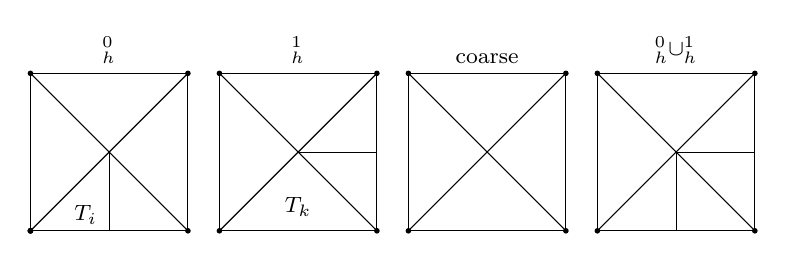
\begin{tikzpicture}[scale=2]
		
		\def \xone{0};
		\def \yone{0};		
		% first rectangle
		\coordinate (A) at (\xone,\yone);
		
        \draw (A) -- ++(0,1) -- ++(1,0)-- ++(0,-1) --cycle;
        \draw (A) -- ++(1,1);
        \draw (A) ++(0,1) -- ++(1,-1);
        \draw (A) ++(0.5,0) -- ++(0,0.5);
        \filldraw (A)         circle (0.4pt);
        \filldraw (A) ++(1,0) circle (0.4pt);
        \filldraw (A) ++(0,1) circle (0.4pt);
        \filldraw (A) ++(1,1) circle (0.4pt);
        
        
        % second rectangle
        \coordinate (A1) at (\xone + 1.2,\yone);
        
        \draw (A1) -- ++(0,1) -- ++(1,0)-- ++(0,-1) --cycle;
        \draw (A1) -- ++(1,1);
        \draw (A1) ++(0,1) -- ++(1,-1);
        \draw (A1) ++(0.5,0.5) -- ++(0.5,0);
        \filldraw (A)         circle (0.4pt);
        \filldraw (A1)         circle (0.4pt);
        \filldraw (A1) ++(1,0) circle (0.4pt);
        \filldraw (A1) ++(0,1) circle (0.4pt);
        \filldraw (A1) ++(1,1) circle (0.4pt);
        
        % third rectangle
        \coordinate (A2) at (\xone + 2.4,\yone);
        
        \draw (A2) -- ++(0,1) -- ++(1,0)-- ++(0,-1) --cycle;
        \draw (A2) -- ++(1,1);
        \draw (A2) ++(0,1) -- ++(1,-1);
        \filldraw (A)         circle (0.4pt);
        \filldraw (A2)         circle (0.4pt);
        \filldraw (A2) ++(1,0) circle (0.4pt);
        \filldraw (A2) ++(0,1) circle (0.4pt);
        \filldraw (A2) ++(1,1) circle (0.4pt);
        
        
        
        % forth rectangle
        \coordinate (A3) at (\xone + 3.6,\yone);
        
        \draw (A3) -- ++(0,1) -- ++(1,0)-- ++(0,-1) --cycle;
        \draw (A3) -- ++(1,1);
        \draw (A3) ++(0,1) -- ++(1,-1);
        \draw (A3) ++(0.5,0) -- ++(0,0.5);
        \draw (A3) ++(0.5,0.5) -- ++(0.5,0);
        \filldraw (A)         circle (0.4pt);
        \filldraw (A3)         circle (0.4pt);
        \filldraw (A3) ++(1,0) circle (0.4pt);
        \filldraw (A3) ++(0,1) circle (0.4pt);
        \filldraw (A3) ++(1,1) circle (0.4pt);
        
        \fill[black,font=\footnotesize] (A)  ++(0.5,1) node[above] {$\T^0_h$}
                                        (A1) ++(0.5,1) node[above] {$\T^1_h$}
                                        (A2) ++(0.5,1) node[above] {coarse}
                                        (A3) ++(0.5,1) node[above] {$\T^0_h \cup \T^1_h $}
                                        (A)  ++(0.35,0.1) node	   {$T_i$}
                                        (A1) ++(0.5,0.15)  node 	   {$T_k$} ;
\end{tikzpicture}

\caption{example of union of multiple meshes}
\label{ch_mult_union}
\end{figure}
	$\implies \T^0_h \cup \T^1_h$ is union of locally finest simplices. The integral is typically computed by using local basisfunctions.\nl
	$\varphi_{i,j}$: $j$-th local basisfunction on $T_i \in \T^0_h$\\
	$\psi_{i,j}$: $j$-th local basisfunction on $T_i \in \T^1_h$\nl
	there are two cases: integral is evaluated on element of $\T^0_h$ or $\T^1_0$.
	\begin{align*}
		\int \limits_{T_i  \in \T^0_h} \psi_{k,l} \varphi_{i,j}
	\end{align*}
	for so,e $l,j$ with elemtn $T_k \in \T^1_h$ with $T_i \subset T_k$. $\implies$ $\psi_{k,l}$ is not a local basisfunction on $T_i$.\nl
	Idea: define $\psi_{k,l}$ as linear combination of local basisfunctions of $T_i$.
	\begin{align*}
		\int \limits_{T \in \T^0_h} \psi_{k,l}\varphi_{i,j} = \int \limits_{T \in \T^0_h} \sum \limits_m \left( c_{k,m} \varphi_{i,m} \right)\varphi_{i,j}
	\end{align*}
	with coefficients $c_{k,m}$. For the other case: 
	\begin{align*}
	\int \limits_{T \in \T^1_h} \psi_{k,l}\varphi_{i,j} = \int \limits_{T \in \T^0_h} \sum \limits_m  \psi_{k,l} \left( c_{k,m} \psi_{i,m} \right)
	\end{align*}
	For the assembly step we use a mesh traverse algorithm which creates requested elements on demand, traverses two meshes in parallel and create union in virtual way.
	\begin{figure}[H]
	\center
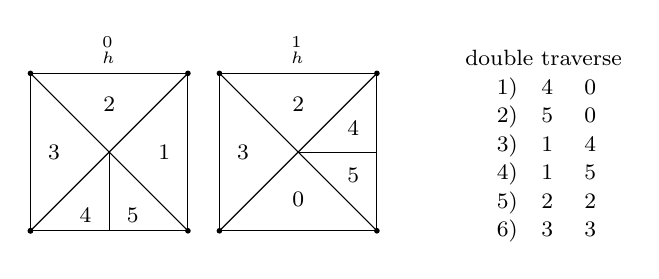
\begin{tikzpicture}[scale=2]
		
		\def \xone{0};
		\def \yone{0};		
		% first rectangle
		\coordinate (A) at (\xone,\yone);
		
        \draw (A) -- ++(0,1) -- ++(1,0)-- ++(0,-1) --cycle;
        \draw (A) -- ++(1,1);
        \draw (A) ++(0,1) -- ++(1,-1);
        \draw (A) ++(0.5,0) -- ++(0,0.5);
        \filldraw (A)         circle (0.4pt);
        \filldraw (A) ++(1,0) circle (0.4pt);
        \filldraw (A) ++(0,1) circle (0.4pt);
        \filldraw (A) ++(1,1) circle (0.4pt);
        
        \fill[black,font=\footnotesize] (A)  ++(0.5,1) node[above] {$\T^0_h$}
        								(A)  ++(0.35,0.1) node	   {$4$}
        								(A)  ++(0.65,0.1) node	   {$5$}
        								(A)  ++(0.15,0.5) node	   {$3$}
        								(A)  ++(0.5,0.8) node	   {$2$}
        								(A)  ++(0.85,0.5) node	   {$1$};
        
        % second rectangle
        \coordinate (A1) at (\xone + 1.2,\yone);
        
        \draw (A1) -- ++(0,1) -- ++(1,0)-- ++(0,-1) --cycle;
        \draw (A1) -- ++(1,1);
        \draw (A1) ++(0,1) -- ++(1,-1);
        \draw (A1) ++(0.5,0.5) -- ++(0.5,0);
        \filldraw (A)         circle (0.4pt);
        \filldraw (A1)         circle (0.4pt);
        \filldraw (A1) ++(1,0) circle (0.4pt);
        \filldraw (A1) ++(0,1) circle (0.4pt);
        \filldraw (A1) ++(1,1) circle (0.4pt);
        
        \fill[black,font=\footnotesize] (A1) ++(0.5,1) node[above] {$\T^1_h$}
        								(A1)  ++(0.85,0.65) node	   {$4$}
        								(A1)  ++(0.85,0.35) node	   {$5$}
        								(A1)  ++(0.15,0.5) node	   {$3$}
        								(A1)  ++(0.5,0.8) node	   {$2$}
        								(A1)  ++(0.5,0.2) node	   {$0$};
        
         % coarse rectangle
%        \coordinate (A2) at (\xone - 1.2,\yone);
        
%        \draw (A2) -- ++(0,1) -- ++(1,0)-- ++(0,-1) --cycle;
%        \draw (A2) -- ++(1,1);
%        \draw (A2) ++(0,1) -- ++(1,-1);
%        \filldraw (A)         circle (0.4pt);
%        \filldraw (A2)         circle (0.4pt);
%        \filldraw (A2) ++(1,0) circle (0.4pt);
%        \filldraw (A2) ++(0,1) circle (0.4pt);
%        \filldraw (A2) ++(1,1) circle (0.4pt);
        
%        \fill[black,font=\footnotesize] (A2) ++(0.5,1) node[above] {coarse}
%        								(A2)  ++(0.5,0.2) node	   {$0$}
%        								(A2)  ++(0.15,0.5) node	   {$3$}
%								        (A2)  ++(0.5,0.8) node	   {$2$}
%        								(A2)  ++(0.85,0.5) node	   {$1$};
        								
        \coordinate (A3) at (\xone + 2.9,\yone);
        \fill[black,font=\footnotesize] (A3) ++(-0.2,1.1) node[right] {double traverse}
        								(A3) ++(0,0.9) 	  node[right] {1)\quad 4 \quad 0}
        								(A3) ++(0,0.72)   node[right] {2)\quad 5 \quad 0}
								        (A3) ++(0,0.54)   node[right] {3)\quad 1 \quad 4}
								        (A3) ++(0,0.36)   node[right] {4)\quad 1 \quad 5}
        								(A3) ++(0,0.18)   node[right] {5)\quad 2 \quad 2}
        								(A3) 			  node[right] {6)\quad 3 \quad 3};
        
\end{tikzpicture}

\caption{double traverse}
\label{ch_mult_traverse}
\end{figure}
	\begin{figure}[H]
	\center
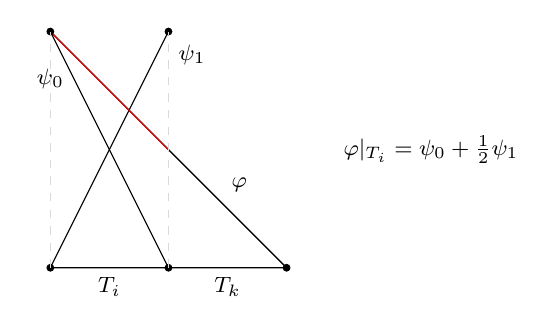
\begin{tikzpicture}[scale=3]
		
		\def \xone{0};
		\def \yone{0};		
		% first rectangle
		\coordinate (A) at (\xone,\yone);
		
        \draw (A) -- ++(1,0) -- ++(-1,1);
        \draw (A) ++(1,0) -- ++(-1,1);
        \draw (A) -- ++(0.5,1);
        \draw (A) ++(0,1) -- ++(0.5,-1);
        \draw[red] (A) ++(0,1) -- ++(0.5,-0.5);
        \filldraw (A)         circle (0.4pt);
        \filldraw (A) ++(1,0) circle (0.4pt);
        \filldraw (A) ++(0,1) circle (0.4pt);
        \filldraw (A) ++(0.5,0) circle (0.4pt);
        \filldraw (A) ++(0.5,1) circle (0.4pt);
        \fill[black,font=\footnotesize] (A) ++(0,0.8)    node {$\psi_0$}
                                        (A) ++(0.6,0.9)  node {$\psi_1$}
                                        (A) ++(0.8,0.35) node {$\varphi$}
                                        (A) ++(1.2,0.5)  node[right] {$\varphi|_{T_i} = \psi_0 + \frac{1}{2}\psi_1$}
                                        (A) ++(0.25,0)   node[below] {$T_i$}
                                        (A) ++(0.75,0)   node[below] {$T_k$};
        \draw[dashed,gray!30!] (A) ++(1/2,0) -- ++(0,1);
        \draw[dashed,gray!30!] (A)			 -- ++(0,1);

        
        
\end{tikzpicture}

\caption{difference of basisfunctions, $T_i \subset T_k$}
\label{ch_mult_other_basis}
\end{figure}
	element matrix $M_{T'}$:(somewhere in this example the dimension of the basis got changed...) 
	\begin{align*}
		M_{T'}&= 
		\begin{pmatrix}
		\int \limits_{T'} \psi_0\varphi_0 & \dots & \int \limits_{T'} \psi_0\varphi_n \\
		\vdots 					 		  & 	  & \vdots\\
		\int \limits_{T'} \psi_n\varphi_0 & \dots & \int \limits_{T'} \psi_n\varphi_n
		\end{pmatrix}\\
		&=
		\begin{pmatrix}
		\int \limits_{T'} \sum \limits_i \left( c_{0i} \varphi_i \right)\varphi_0 & \dots & \int \limits_{T'} \sum \limits_i\left( c_{0i} \varphi_i \right)\varphi_n \\
		\vdots 					 		  & 	  & \vdots\\
		\int \limits_{T'} \sum \limits_i\left( c_{ni} \varphi_i \right)\varphi_0 & \dots & \int \limits_{T'} \sum \limits_i\left( c_{ni} \varphi_i \right)\varphi_n
		\end{pmatrix}\\
		&= C 
		\begin{pmatrix}
		\int \limits_{T'} \varphi_0\varphi_0 & \dots & \int \limits_{T'} \varphi_0\varphi_n \\
		\vdots 					 		  & 	  & \vdots\\
		\int \limits_{T'} \varphi_n\varphi_0 & \dots & \int \limits_{T'} \varphi_n\varphi_n
		\end{pmatrix}
	\end{align*}
	the other case leads to $M_{T'} = (\dots) C^T$.\\
	(PhD thesis Sigi Ling 2016 )
\end{example}
